\documentclass[12pt, conference, compsoc, onecolumn]{IEEEtran}
\usepackage{graphicx}
\usepackage{listings}
\usepackage{array, float}
\usepackage[colorlinks=true]{hyperref}
\usepackage[style=numeric,backend=bibtex]{biblatex}
\graphicspath{ {./figures/} }
\addbibresource{refs.bib}

\lstdefinestyle{model_arch}{
	backgroundcolor=\color{white},   
	basicstyle=\ttfamily,
	breaklines=true,
	showstringspaces=false,
	frame=single, % This adds a box around all sides of the snippet
	rulecolor=\color{black}, % You can specify the color of the box
}

\begin{document}
	\title{ECE1512 - Digital Image Processing and Applications - Project B}
	\author{Swapnil Patel - 999728870 - \today}
	
	\author{\IEEEauthorblockN{Swapnil Patel}
		\IEEEauthorblockA{
			University of Toronto\\
			swap.patel@mail.utoronto.ca\\
			Code: \href{https://github.com/Swapnil949/ECE1512\_2024F\_ProjectRepo\_SwapnilPatel}{Swapnil949/ECE1512\_2024F\_ProjectRepo\_SwapnilPatel}
	}}
	
	\maketitle
	
	\section{State Space Models (SSMs) - Mamba: Linear-Time Sequence Modeling with Selective State Spaces}
	In this section, Mamba, as introduced in the paper "Mamba: Linear-Time Sequence Modeling with Selective State Spaces" \cite{gu2024mamba}, is discussed. Mamba is a novel sequence modeling architecture that leverages Selective State Space Models (SSMs) to address the computational inefficiencies of Transformers while maintaining their ability to perform complex reasoning. The architecture introduces input-dependent dynamics in SSM parameters, enabling selective propagation or forgetting of information along sequences.
	
	This work represents a significant step forward in designing models that combine efficiency and performance, achieving \textbf{linear scaling} in sequence length and demonstrating up to 5× higher inference throughput compared to Transformers. Mamba eliminates the need for attention or MLP blocks, offering a simplified design suitable for multimodal tasks. It achieves state-of-the-art results across various domains, including language, audio, and genomics, and matches the performance of Transformers twice its size in language modeling tasks.
	
	Mamba is designed to solve the computational inefficiency and scalability issues of Transformers, particularly for handling long sequence data across various modalities (e.g., language, audio, and genomics). The primary challenges that Mamba aims to address are:
	
	\subsubsection*{Inefficiency of Self-Attention in Transformers}
	\begin{itemize}
		\item \textbf{Quadratic Complexity:} The self-attention mechanism in Transformers scales quadratically with sequence length, making it computationally expensive and memory-intensive for long sequences \cite{vaswani2023attentionneed}.
		\item \textbf{Limited Context:} Transformers can only process a finite context window efficiently, which limits their ability to model long-range dependencies.
	\end{itemize}
	
	\subsubsection*{Limitations of Existing Efficient Architectures}
	\begin{itemize}
		\item Several subquadratic-time models (e.g., linear attention \cite{katharopoulos2020transformersrnnsfastautoregressive}, gated convolution \cite{rao2022hornetefficienthighorderspatial}, recurrent models \cite{bulatov2022recurrentmemorytransformer}, and structured state space models \cite{gu2022efficientlymodelinglongsequences}) have been proposed to improve efficiency. However they have their own drawbacks. 
		\begin{itemize}
			\item They often fail to match the performance of Transformers, especially in discrete and information-dense data such as natural language.
			\item They lack content-based reasoning capabilities, which are crucial for tasks like language modeling and in-context learning.
			
		\end{itemize}
		
	\end{itemize}
	
	The author's key contribution to State Space models are threefold:
	\begin{enumerate}
		\item \textbf{Selection Mechanism:} A key limitation of previous models was their inability to perform input-dependent selection, crucial for focusing on relevant information and ignoring irrelevant data. To address this, the authors parameterize SSMs based on input, enabling the model to selectively retain or discard information. This mechanism is validated on synthetic tasks such as selective copying and induction heads.
		
		\item \textbf{Hardware-aware Algorithm:} The input-dependent nature of Selective SSMs posed computational challenges. The authors introduce a \textbf{hardware-efficient recurrent algorithm} that leverages a scan operation instead of convolutions, avoiding the need to materialize large intermediate states in GPU memory. This implementation achieves true linear scaling in sequence length and is up to 3× faster than previous SSM methods on modern hardware.
		
		\item \textbf{Simplified Architecture:} By combining the principles of previous SSM architectures with the MLP block of Transformers, the authors design a unified, homogenous block for the Mamba architecture. This streamlined design effectively integrates selective state spaces while maintaining simplicity and scalability.
	\end{enumerate}
	
	\subsection{Mamba Architecture}
	
	The Mamba architecture builds on Selective State Space Models (SSMs) with the following architectural innovations: enhanced selection strategies, hardware-aware computational algorithms, and a simplified yet powerful block design. These advancements enable Mamba to efficiently handle long sequences with linear scaling, achieving performance on par with or surpassing Transformers.
	
	\subsubsection{Selection strategy}
	To improve the selection strategy, Mamba transitions SSMs from time-invariant to time-varying dynamics. This is achieved by making parameters such as $B$, $C$, $\Delta$ input-dependent, allowing the model to selectively propagate or ignore information along the sequence based on its content. This is presented in Algorithm 2 in the paper \cite{gu2022efficientlymodelinglongsequences}. This content-aware parameterization empowers the model to dynamically focus on relevant inputs while filtering out irrelevant ones, improving its ability to handle tasks requiring context sensitivity and reasoning. Such selective capabilities are particularly effective for tasks like selective copying and induction heads, where traditional SSMs face limitations.
	
	\subsubsection{Hardware-aware algorithm}
	The introduction of input-dependent parameters posed computational challenges, addressed by Mamba through a hardware-aware algorithm designed to optimize execution on modern GPUs. Instead of using convolutions, Mamba employs a parallel scan operation to compute recurrently while avoiding materializing large intermediate states in GPU memory. This approach incorporates kernel fusion to reduce memory IO, leverages faster memory levels (e.g., SRAM over HBM), and uses recomputation techniques to minimize memory requirements during backpropagation. These optimizations ensure that Mamba achieves true linear scaling in sequence length and demonstrates up to 3× faster performance compared to previous SSM implementations on hardware such as the NVIDIA A100 GPU.
	
	Together these two innovations create selective SSM which can be used like self-attention to create Mamba block shown in Figure \ref{fig:mamba_arch}.
	\begin{figure}[H]
		\centering
		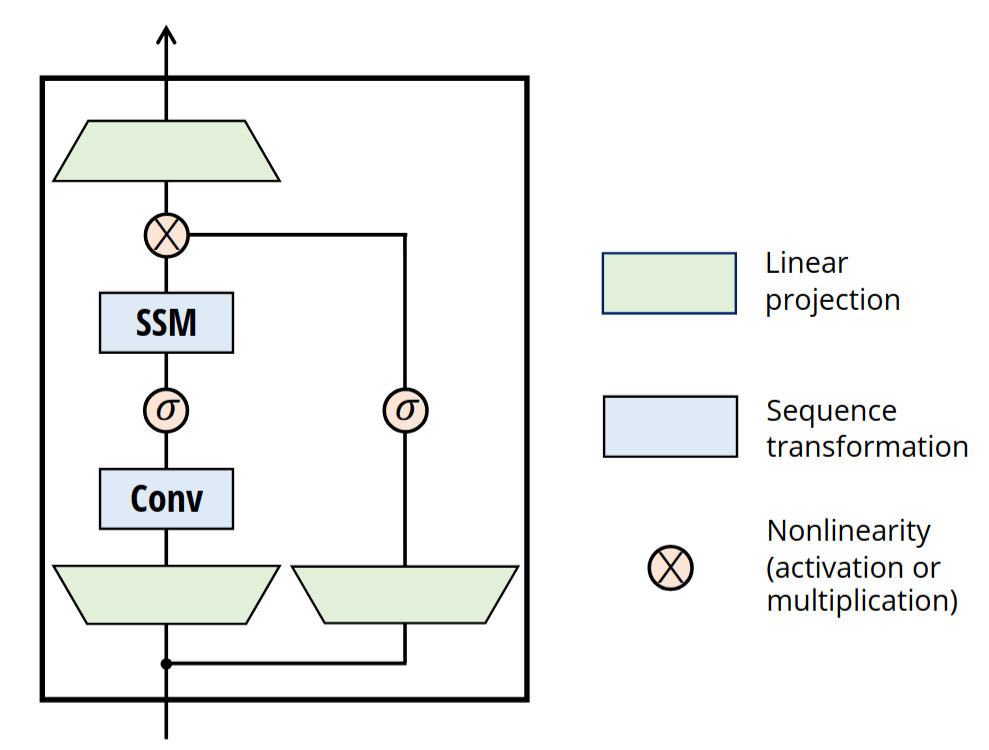
\includegraphics[width=0.48\textwidth]{figures/mamba_arch.png}
		\caption{Mamba Architecture\cite{gu2024mamba}}
		\label{fig:mamba_arch}
	\end{figure}
	
	\subsection{Future Improvements with Mamba}
	The Mamba architecture opens new avenues for enhancements by leveraging emerging techniques developed for Transformer-based models. Through the connection between State Space Models (SSMs) and attention mechanisms established in the SSD framework (Mamba-2) \cite{dao2024transformersssmsgeneralizedmodels}, researchers can adapt and extend Transformer innovations to Mamba, paving the way for significant advancements in its application and utility. Two key areas for future exploration include parameter-efficient fine-tuning and mitigation of catastrophic forgetting.
	
	\subsubsection*{Parameter-Efficient Fine-Tuning}
	
	As large foundation models scale to billions of parameters, fine-tuning them for specific downstream tasks becomes computationally expensive and resource-intensive. Techniques like Low-Rank Adaptation (LoRA) and Adapters have emerged as efficient alternatives, enabling rapid and cost-effective fine-tuning by adjusting only a small subset of model parameters. Adopting these techniques for Mamba models could significantly broaden their usability across diverse domains. For instance, LoRA can facilitate efficient fine-tuning for SSD models, reducing computational overhead while maintaining performance. However, the integration of PEFT techniques into Mamba-based models remains an open area for further investigation.
	
	\subsubsection*{Mitigation of Catastrophic Forgetting}
	
	Catastrophic forgetting—where a model loses performance on previously learned tasks when exposed to new ones—poses a challenge for foundation models, including Mamba. Addressing this issue is essential for ensuring Mamba's reliability across pretraining and downstream tasks. Emerging solutions, such as Reward Maximization and Distribution Matching strategies, as well as continual learning techniques developed for Transformers, offer promising approaches to mitigate forgetting in Mamba models. By connecting SSMs and attention, these techniques could be adapted for Mamba, but their application requires further exploration to realize their full potential.
	
	\newpage
	\subsection{MambaVision}
	
	Mamba is excellent for sequence modeling tasks such as language processing, audio, and genomics, however it faces challenges when applied to vision tasks. This is due to its autoregressive nature, which limits its ability to efficiently capture global spatial dependencies. Vision tasks require simultaneous understanding of both local pixel-level interactions and global spatial relationships, which are not inherently modeled in Mamba's sequential SSM framework.
	
	To address these limitations, MambaVision \cite{hatamizadeh2024mambavision} introduces a hybrid architecture that combines the efficiency of Mamba's SSMs with the global modeling capabilities of Transformers. By retaining Mamba's core principles and incorporating key modifications, such as convolutional layers for local feature extraction and Transformer blocks for capturing long-range spatial dependencies, MambaVision is specifically designed to meet the demands of vision applications effectively.
	\\
	
	Key innovations in MambaVision are:
	\subsubsection*{Hybrid Architecture}
	\begin{itemize}
		\item MambaVision employs a multi-resolution hierarchical structure with four stages:
		\begin{itemize}
			\item Stages 1 and 2 use convolutional layers for fast local feature extraction at high resolutions.
			\item Stages 3 and 4 combine MambaVision Mixer blocks (based on SSMs) with Transformer blocks to capture long-range dependencies.
		\end{itemize}
		\item This design ensures both local and global spatial relationships are effectively modeled.
	\end{itemize}
	
	\subsubsection*{Redesigned Mamba Blocks}
	\begin{itemize}
		\item MambaVision replaces causal convolutions with regular convolutions to remove directional constraints unsuitable for spatial data.
		\item A symmetric branch without SSMs is added to enhance global context modeling, with outputs from both branches concatenated for richer feature representation.
	\end{itemize}
	
	\subsubsection*{Transformer Integration}
	\begin{itemize}
		\item Self-attention blocks are incorporated in the final layers of the architecture, enabling the model to recover lost global context and better capture long-range spatial dependencies.
	\end{itemize}
	
	
	The resultant MambaVision architecture is depicted in Figure \ref{fig:mambavision_arch}.

	\begin{figure}[H]
		\centering
		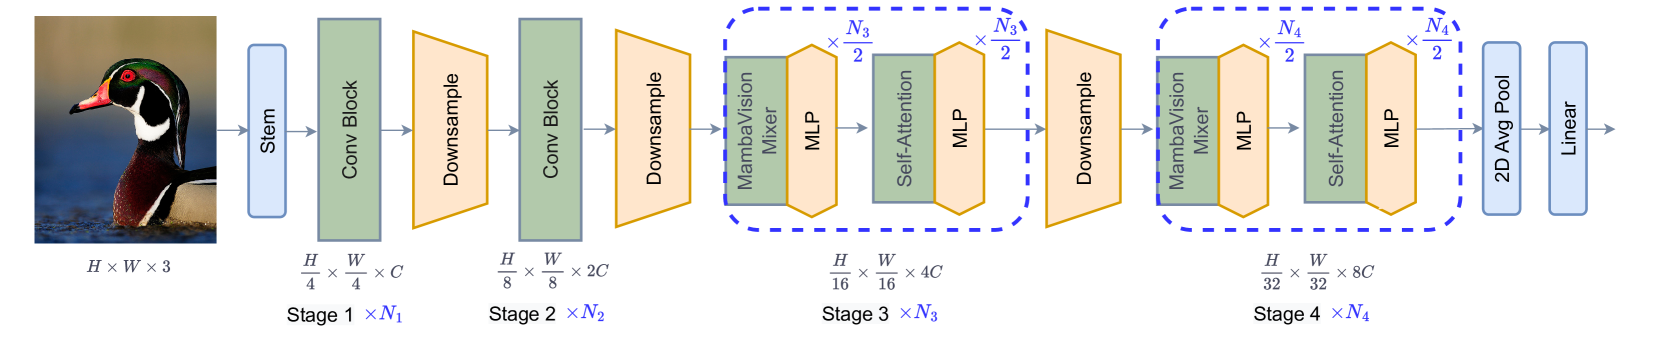
\includegraphics[width=0.99\textwidth]{figures/mambavision_arch.png}
		\caption{Mambavision Architecture\cite{hatamizadeh2024mambavision}}
		\label{fig:mambavision_arch}
	\end{figure}
	
	MambaVision achieves state-of-the-art performance across various vision tasks by effectively balancing accuracy and computational efficiency. In image classification, it achieves optimum tradeoff for Top-1 accuracy and throughput on the ImageNet-1K dataset, outperforming both Transformer-based and convolutional backbones. Additionally, in object detection and segmentation tasks, MambaVision surpasses comparably sized models on benchmarks such as MS COCO and ADE20K, demonstrating superior performance in instance segmentation and semantic segmentation, thereby validating its versatility and efficiency as a vision backbone.
	
	\subsubsection{Experiment}
	\hfill\\
	
	To evaluate the adaptability and performance of MambaVision in vision tasks, an experiment was conducted by fine-tuning the MambaVision model and a standard Vision Transformer (ViT) on the CIFAR-100 dataset \cite{Krizhevsky09cifar100} shown in Figure \ref{fig:cifar100}. This dataset, comprising 100 classes of diverse object categories, serves as an ideal benchmark for assessing a model's capability to handle fine-grained image classification. The experiment aimed to compare the effectiveness of the hybrid MambaVision architecture against the established ViT framework in terms of classification accuracy and computational efficiency, providing insights into their relative strengths in processing high-dimensional visual data.
	
	\begin{figure}[H]
		\centering
		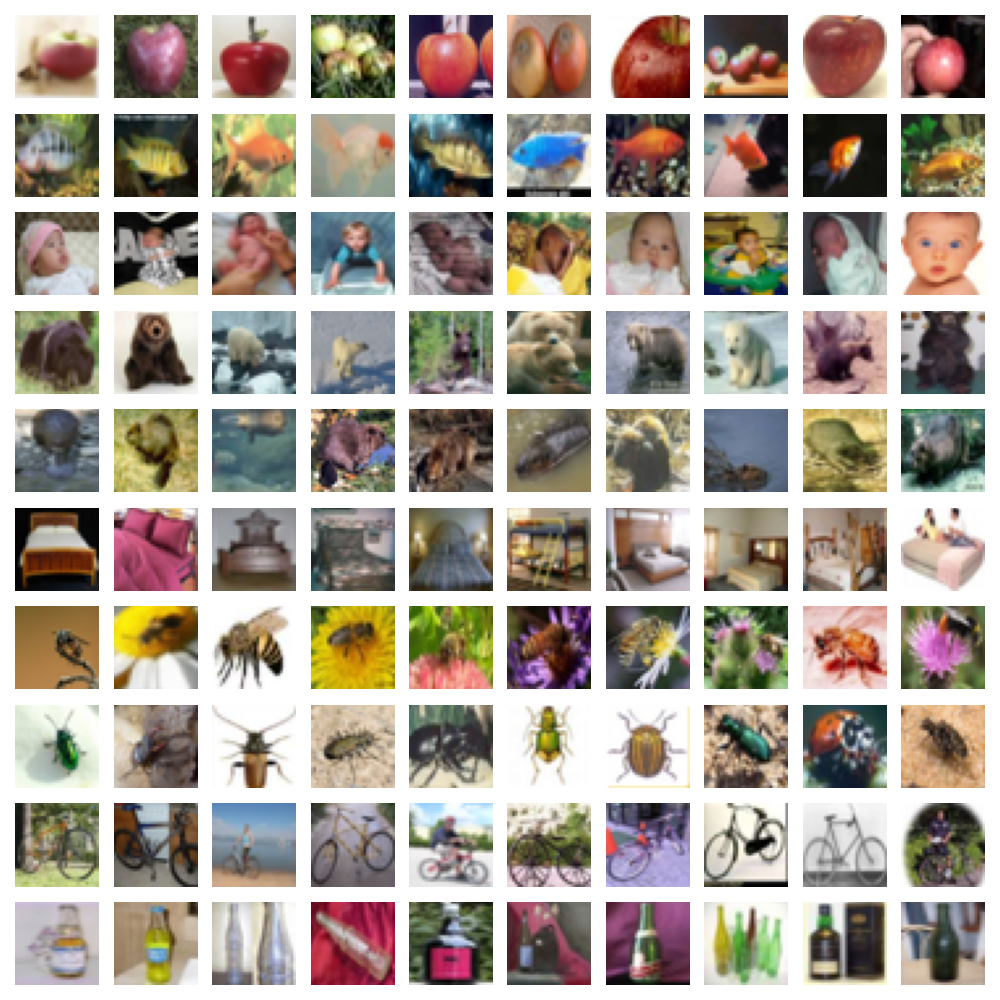
\includegraphics[width=0.73\textwidth]{figures/cifar100_sample.png}
		\caption{Sample of CIFAR100 Dataset\cite{Krizhevsky09cifar100}}
		\label{fig:cifar100}
	\end{figure}
	

	For this experiment, the \textbf{google/vit-base-patch16-224} \cite{wu2020visual} model with 86.6 million parameters and the \textbf{nvidia/MambaVision-B-1K} \cite{hatamizadeh2024mambavision} model with 97.7 million parameters were fine-tuned for the selected dataset. Since both models were originally trained on ImageNet-1k data with 1000 image classes, slight adaptations were made to fine-tune them on CIFAR-100, which contains only 100 image classes. The model selection ensures a fair comparison, given their similar scale. The fine-tuning code can be found in the supplementary GitHub repository.
	
	\hfill\\
	Figure \ref{fig:finetune} shows the training and test accuracies for the fine-tuning stages of both models. ViT slightly outperforms in terms of both training and test accuracy, reflecting its status as a leading solution for image classification problems due to its Transformer architecture. However, MambaVision's accuracy is very close, indicating strong performance as well
	
	\begin{figure}[H]
		\centering
		% First figure
		\begin{minipage}{0.49\textwidth}
			\centering
			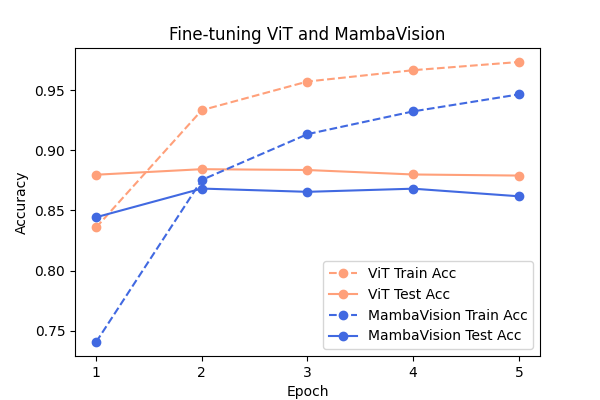
\includegraphics[width=\linewidth]{figures/fine_tuning.png}
			\caption{Fine-tuning ViT and MambaVision for CIFAR100}
			\label{fig:finetune}
		\end{minipage}
		\hfill
		% Second figure
		\begin{minipage}{0.49\textwidth}
			\centering
			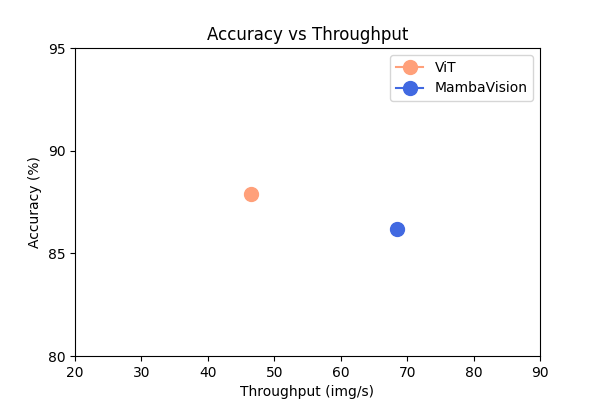
\includegraphics[width=\linewidth]{figures/accuracy_vs_throughput.png}
			\caption{Inference Accuracy and Throughput for fine-tuned models}
			\label{fig:acc_throughput}
		\end{minipage}
	\end{figure}
	
	However, the advantages of MambaVision become apparent when examining the results during the inference stage. For this purpose, inference was profiled using the CIFAR-100 test dataset. Figure \ref{fig:acc_throughput} compares the accuracy and image throughput during inference. As shown in the figure, MambaVision achieves approximately 85\% test accuracy while maintaining a throughput of 68 images/sec. In contrast, ViT achieves around 87\% test accuracy but has a lower image throughput of only 45 images/sec. The tests were conducted using an \texttt{Nvidia 4090 GPU}.
	
	Despite the slightly larger size of the MambaVision base model compared to the ViT base model, it achieves higher throughput while maintaining comparable test accuracies, highlighting the advantages of the Mamba Architecture.
	
	\subsection{Parameter-Efficient Fine Tuning for Mamba - LoRa}
	\begin{figure}[H]
		\centering
		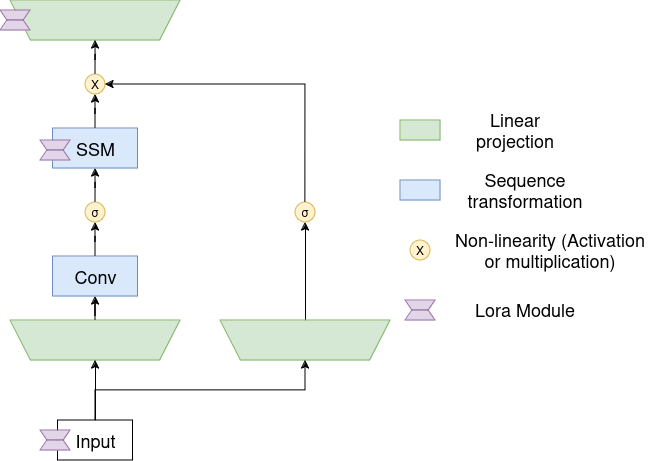
\includegraphics[width=0.73\textwidth]{figures/lora_mamba.png}
		\caption{Proposed Parameter-Efficient Fine Tuning for Mamba using LoRA}
		\label{fig:lora_mamba}
	\end{figure}
	
	\newpage
	\section{Vision Language Models (VLMs) - LLaVA: Large Language and Vision Assistant}
	
	In this section, LLaVA (Large Language and Vision Assistant), as presented in the paper "Visual Instruction Tuning" \cite{liu2023llava}, is discussed. LLaVA is an end-to-end trained multimodal AI system that connects a vision encoder with a large language model (LLM) to interpret and follow human instructions involving both visual and linguistic contexts. The work in this paper represents the first attempt to use language-only GPT-4 to generate multimodal language-image instruction-following data, enabling instruction tuning for multimodal tasks.
	
	The paper demonstrates that LLaVA achieves remarkable capabilities in multimodal chat, often exhibiting behaviors similar to multimodal GPT-4 on unseen images and instructions. Evaluations show an 85.1\% relative score compared to GPT-4 on a synthetic multimodal instruction-following dataset. Furthermore, when fine-tuned on ScienceQA, LLaVA achieves a new state-of-the-art accuracy of 92.53\%, highlighting its effectiveness in reasoning and answering visual and textual queries. To facilitate further research, the authors release the GPT-4-generated visual instruction tuning data, their model, and associated codebase to the public.
	
	\subsection{LLaVA Architecture}
	\begin{figure}[H]
		\centering
		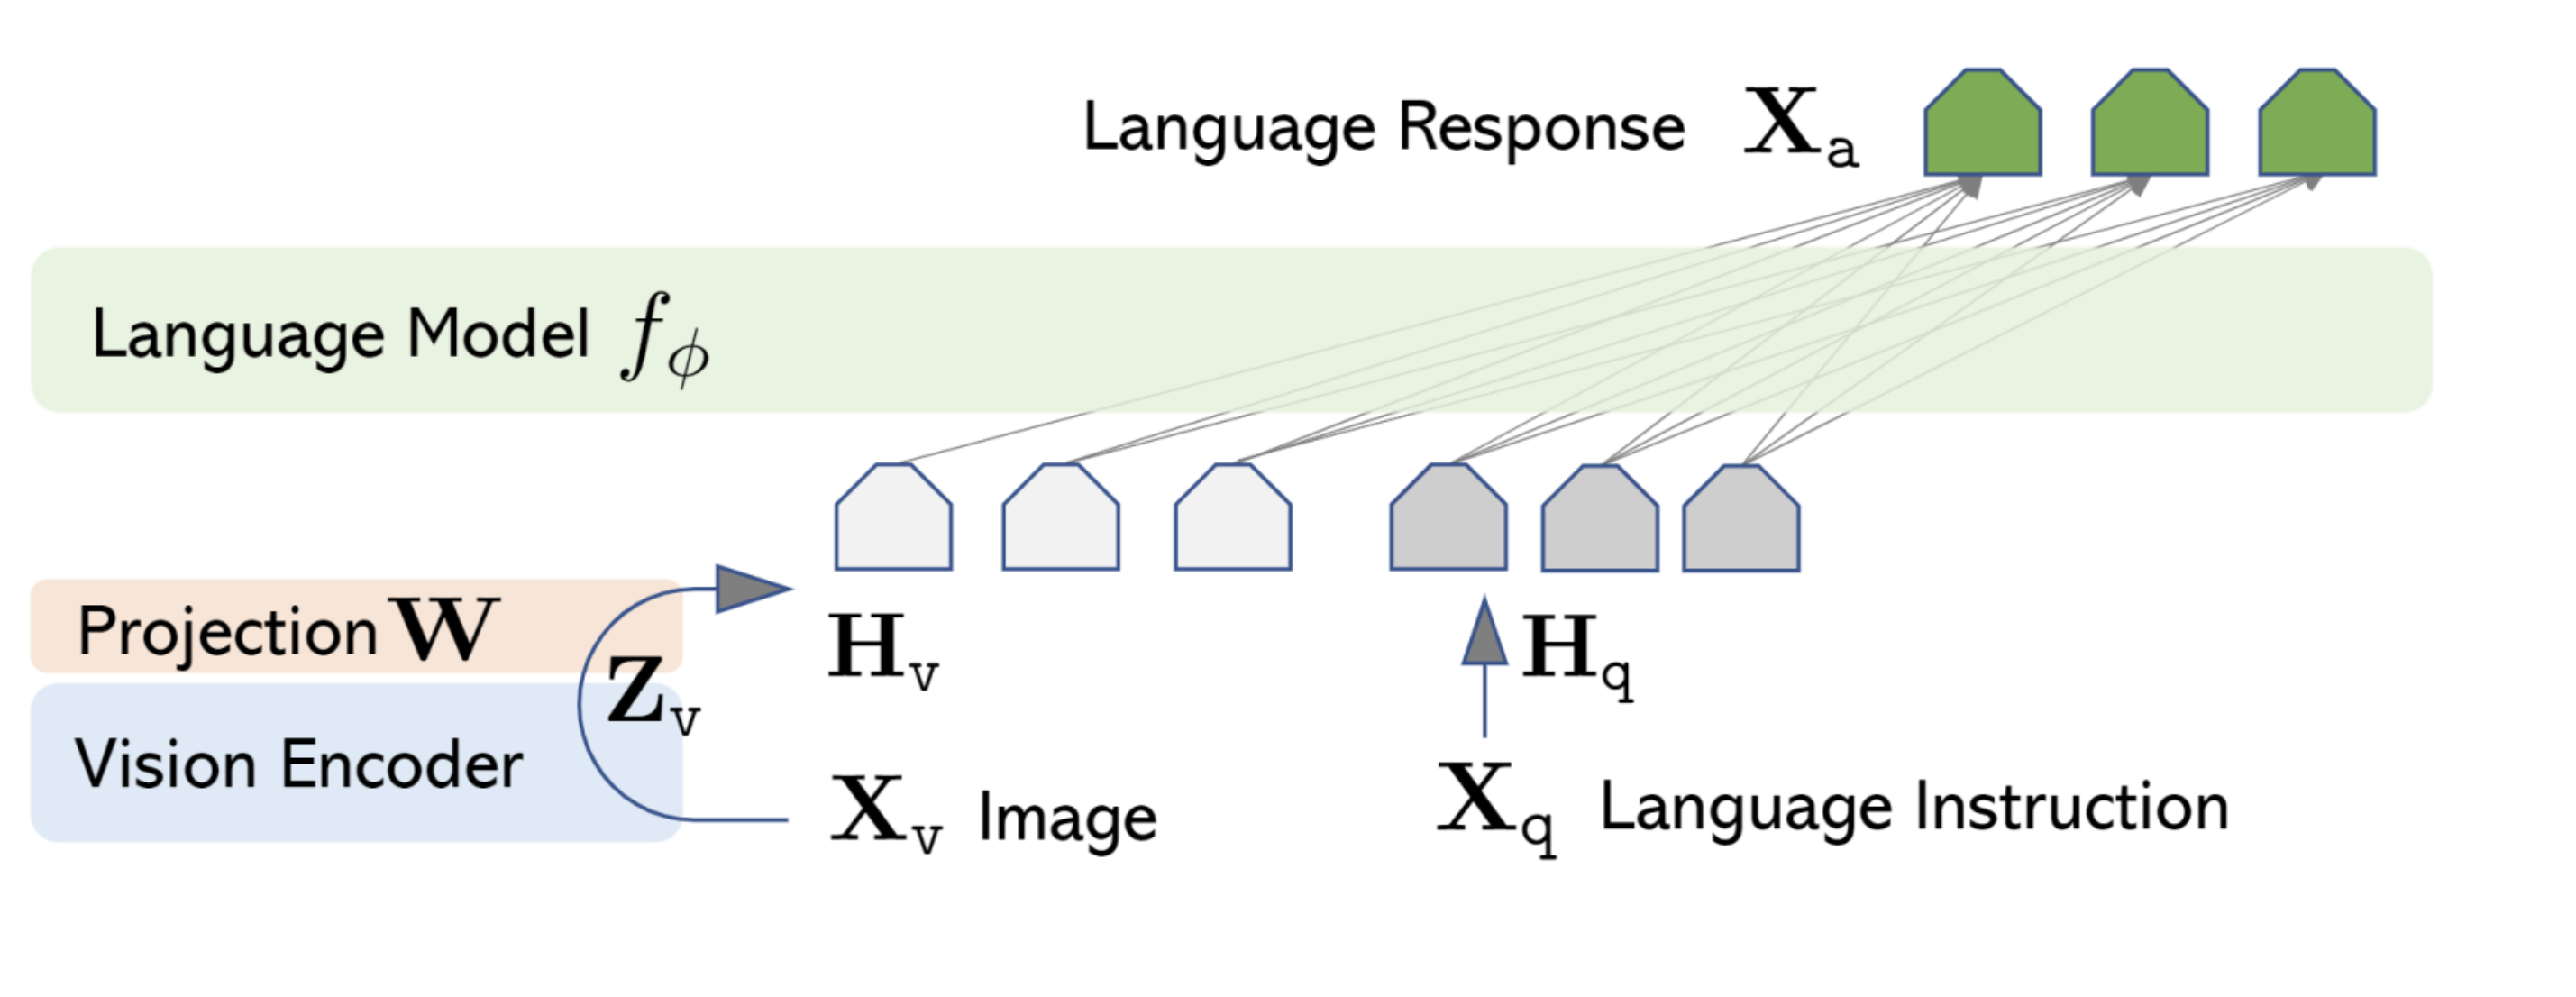
\includegraphics[width=0.75\textwidth]{figures/conceptual-diagram-of-llava.png}
		\caption{LLaVA Architecture \cite{liu2023llava}}
		\label{fig:llava_arch}
	\end{figure}
	
	The LLaVA (Large Language and Vision Assistant) model architecture is designed to integrate visual and linguistic modalities to enable advanced multimodal understanding. Its structure consists of several key components, which work together to process both image and text inputs, generating coherent and context-aware responses.
	\subsubsection*{Vision Encoder} 
	At the foundation of the architecture is the Vision Encoder, which processes the input image $X_v$. This encoder (e.g., CLIP) transforms the raw image data into a high-dimensional feature representation $H_v$. These features encapsulate the visual information in a format suitable for downstream processing.
	
	\subsubsection*{Projection Layer} 
	The Projection Layer serves as a critical bridge between the Vision Encoder and the Language Model. It applies a projection matrix $W$ to convert the feature representations $H_v$ into a format $Z_v$ that is compatible with the language model's embedding space. This alignment ensures seamless integration of visual data with textual data for joint processing.
	
	\subsubsection*{Language Instruction Input}
	Alongside the visual input, the model receives a Language Instruction input $X_q$, which represents the textual task or query. This input is processed by the language model to generate its own feature representation $H_q$, encapsulating the semantic meaning of the query.
	
	\subsubsection*{Language Model}
	At the core of the architecture is the Language Model $f_\phi$, which is a pre-trained large language model (e.g., Vicuna). This model takes both the projected visual features $Z_v$ and the linguistic features $H_q$ as input, integrating them to produce a unified understanding of the multimodal context.
	
	\subsubsection*{Output Generation}
	The final output, $X_a$, is a language-based response that incorporates information from both the visual and textual inputs. This response can range from answering specific questions about an image to providing detailed descriptions or engaging in complex reasoning tasks that require a multimodal perspective.
	
	
	\section*{References}
	\addcontentsline{toc}{section}{\protect\numberline{}References}
	\nocite{*}
	\printbibliography[heading=none]
	
	%	\onecolumn
	%	\section*{Appendix}
	%	\addcontentsline{toc}{section}{\protect\numberline{}Appendix}
	
	
\end{document}